\documentclass{mylib/reporteConCalif}
\graphicspath{ {img/labdise_pract8/} }
\usepackage{float}
\usepackage{float}
\usepackage{subfig}
\title{Reporte}
\author{rodrigofranciscopablo }

\subject{Laboratorio de Diseño Digital}
\mytitle{Reporte de práctica 8}
\mysubTitle{Decodificador utilizando mediana escala de integración}
\students{Francisco Pablo \textsc{Rodrigo}}
\teacher{M.I. Guevara Rodríguez \textsc{Ma. del Socorro}}
\group{6}
\deliverDate{23 de abril de 2019}

\begin{document}

\coverPage

\section{Objetivos}

\subsection{General}

El alumno diseñará circuitos combinacionales.

\subsection{Particular}

El alumno analizará, diseñará e implementará decodificadores en mediana escala de integración.
\section{Introducción}

Un decodificador es un circuito integrado que genera todos los minitérminos correspondientes a n entradas.Cada salida corresponde a un minitérmino, empezando con la salida superior que corresponde al minitérmino 0. Como se muestra en la siguiente figura.

\insertImage{dec1}{Ejemplo de decodificador}{4}

En la practica, la mayoría de los decodificadores tienen las salidas complementadas indicándolo mediante una pequeña burbuja o circulo en la salida, es decir, el decodificador genera maxitérminos(0) en lugar de minitérminos(1).

Una de las aplicaciones de un decodificador es la implementación de funciones Booleanas. Una función Booleana de n variables puede ser implementada fácilmente al unir los minitérminos(maxitérminos) correspondientes a la función utilizando una compuerta OR(NAND).


\newpage
\section{Previo}

\newpage
\section{Desarrollo}

Para esta práctica tuvimos que diseñar dos decodificadores de 3x8 e intentamos conectarlos entre ellos de manera que pudieran funcionar como uno solo para que pudieran controlar un display de 7 segmentos.

Para conectarlos hicimos uso de señal \textit{enable} de cada uno de nuestros decodificadores.

\begin{figure}[H]%
    \centering
    \subfloat[Cero]{{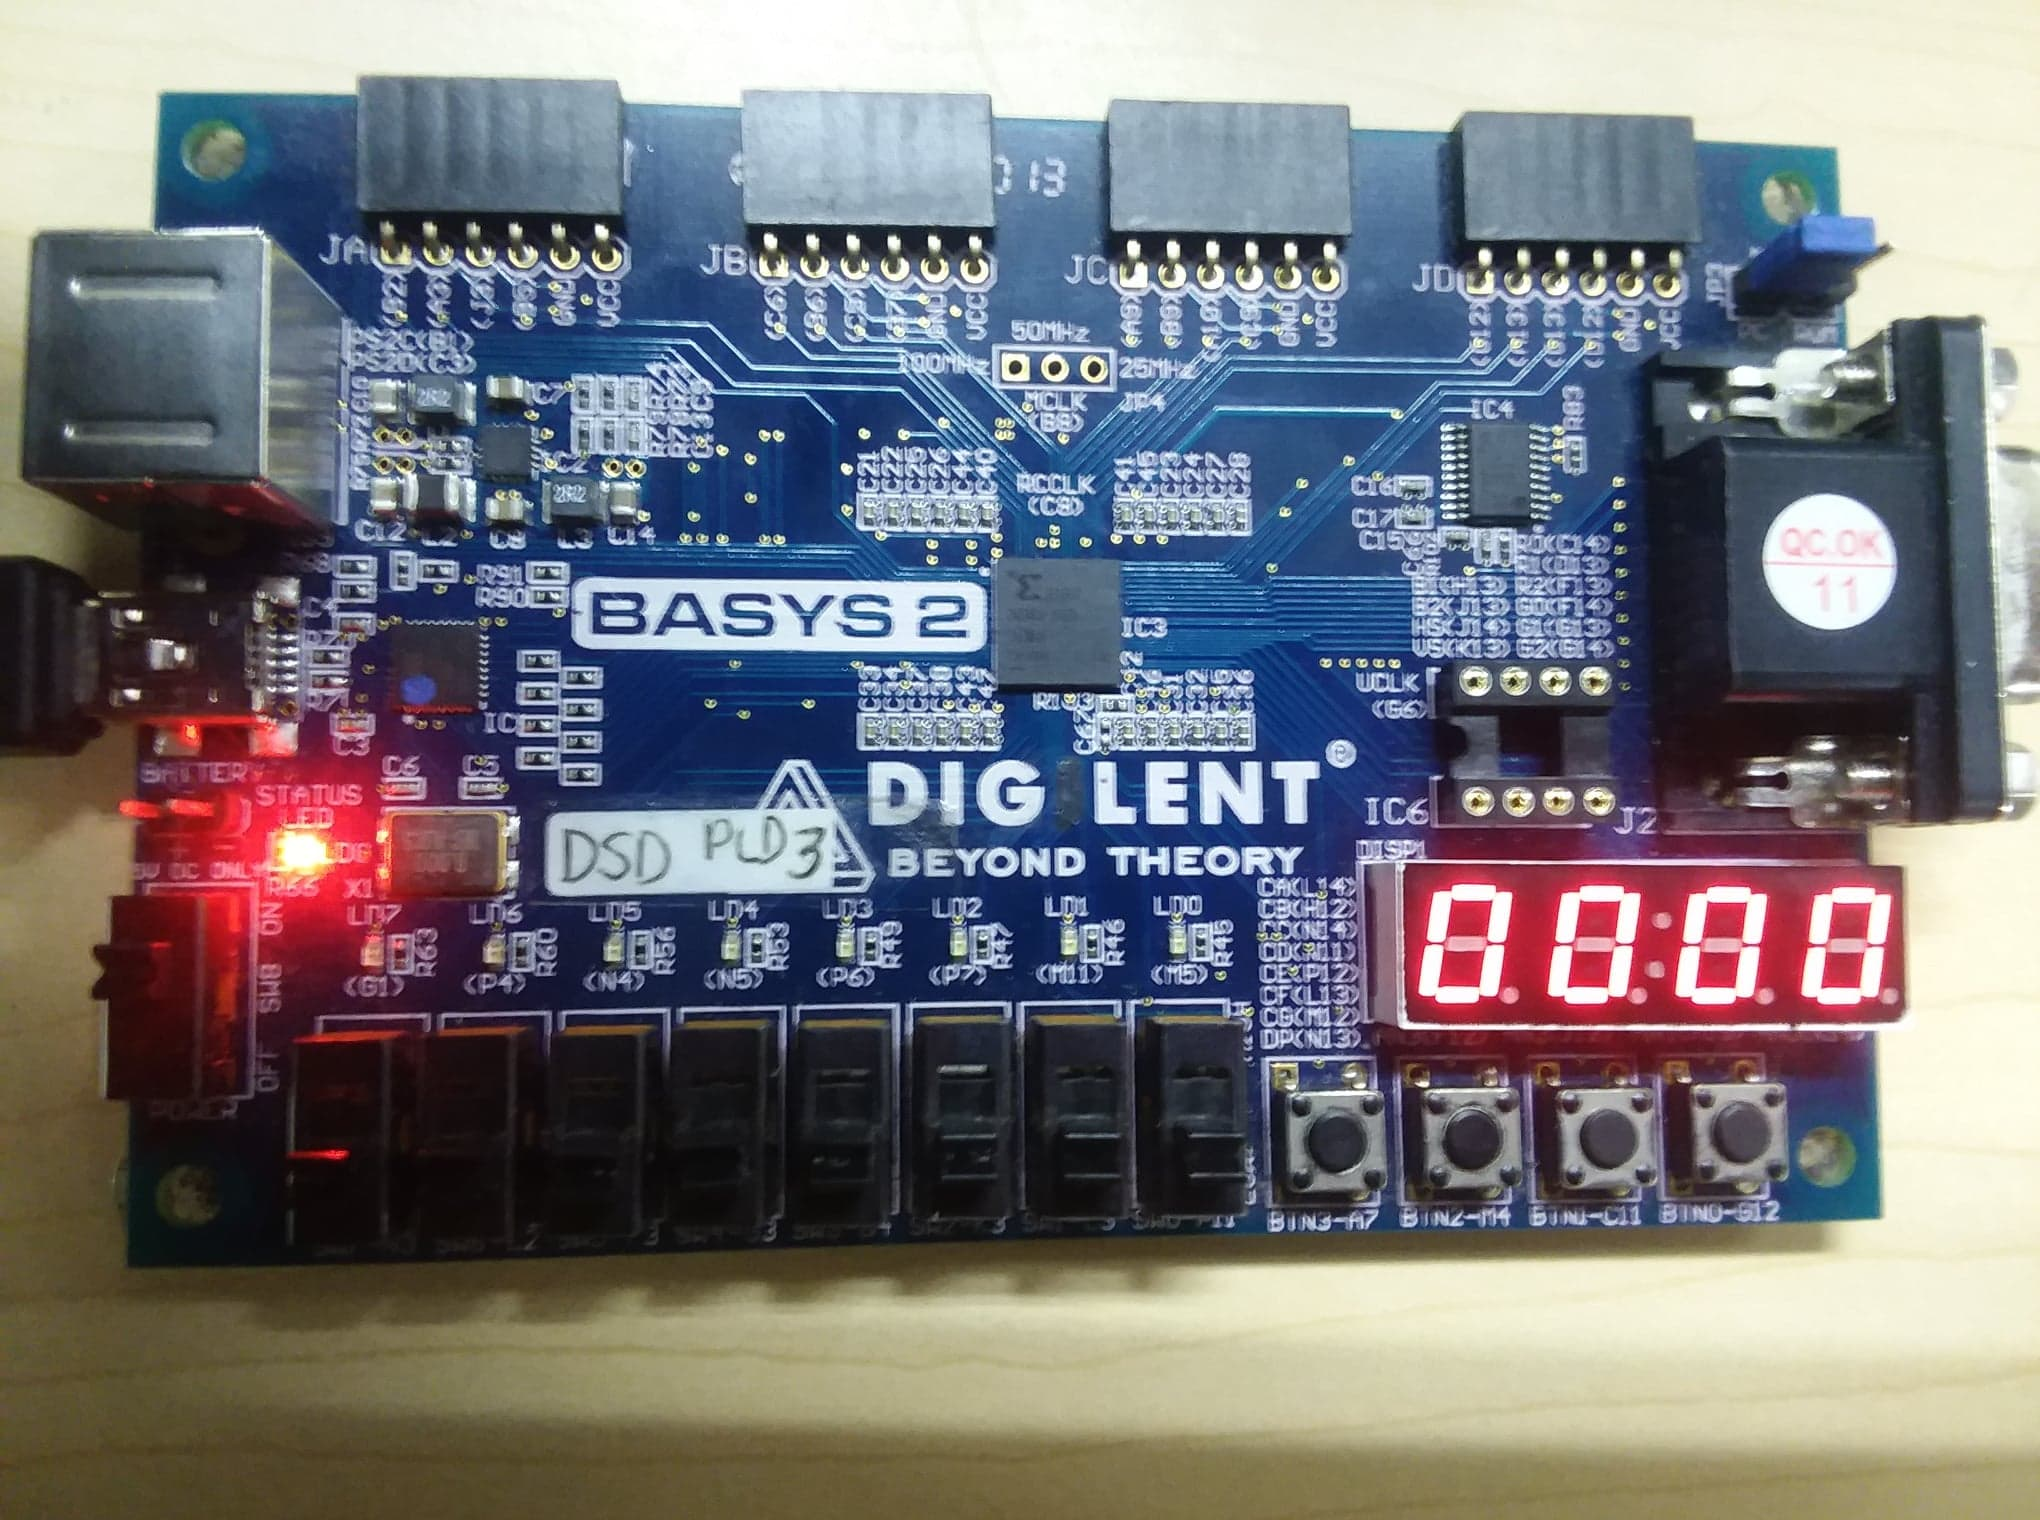
\includegraphics[width=7cm]{00} }}%
    \qquad
    \subfloat[Uno]{{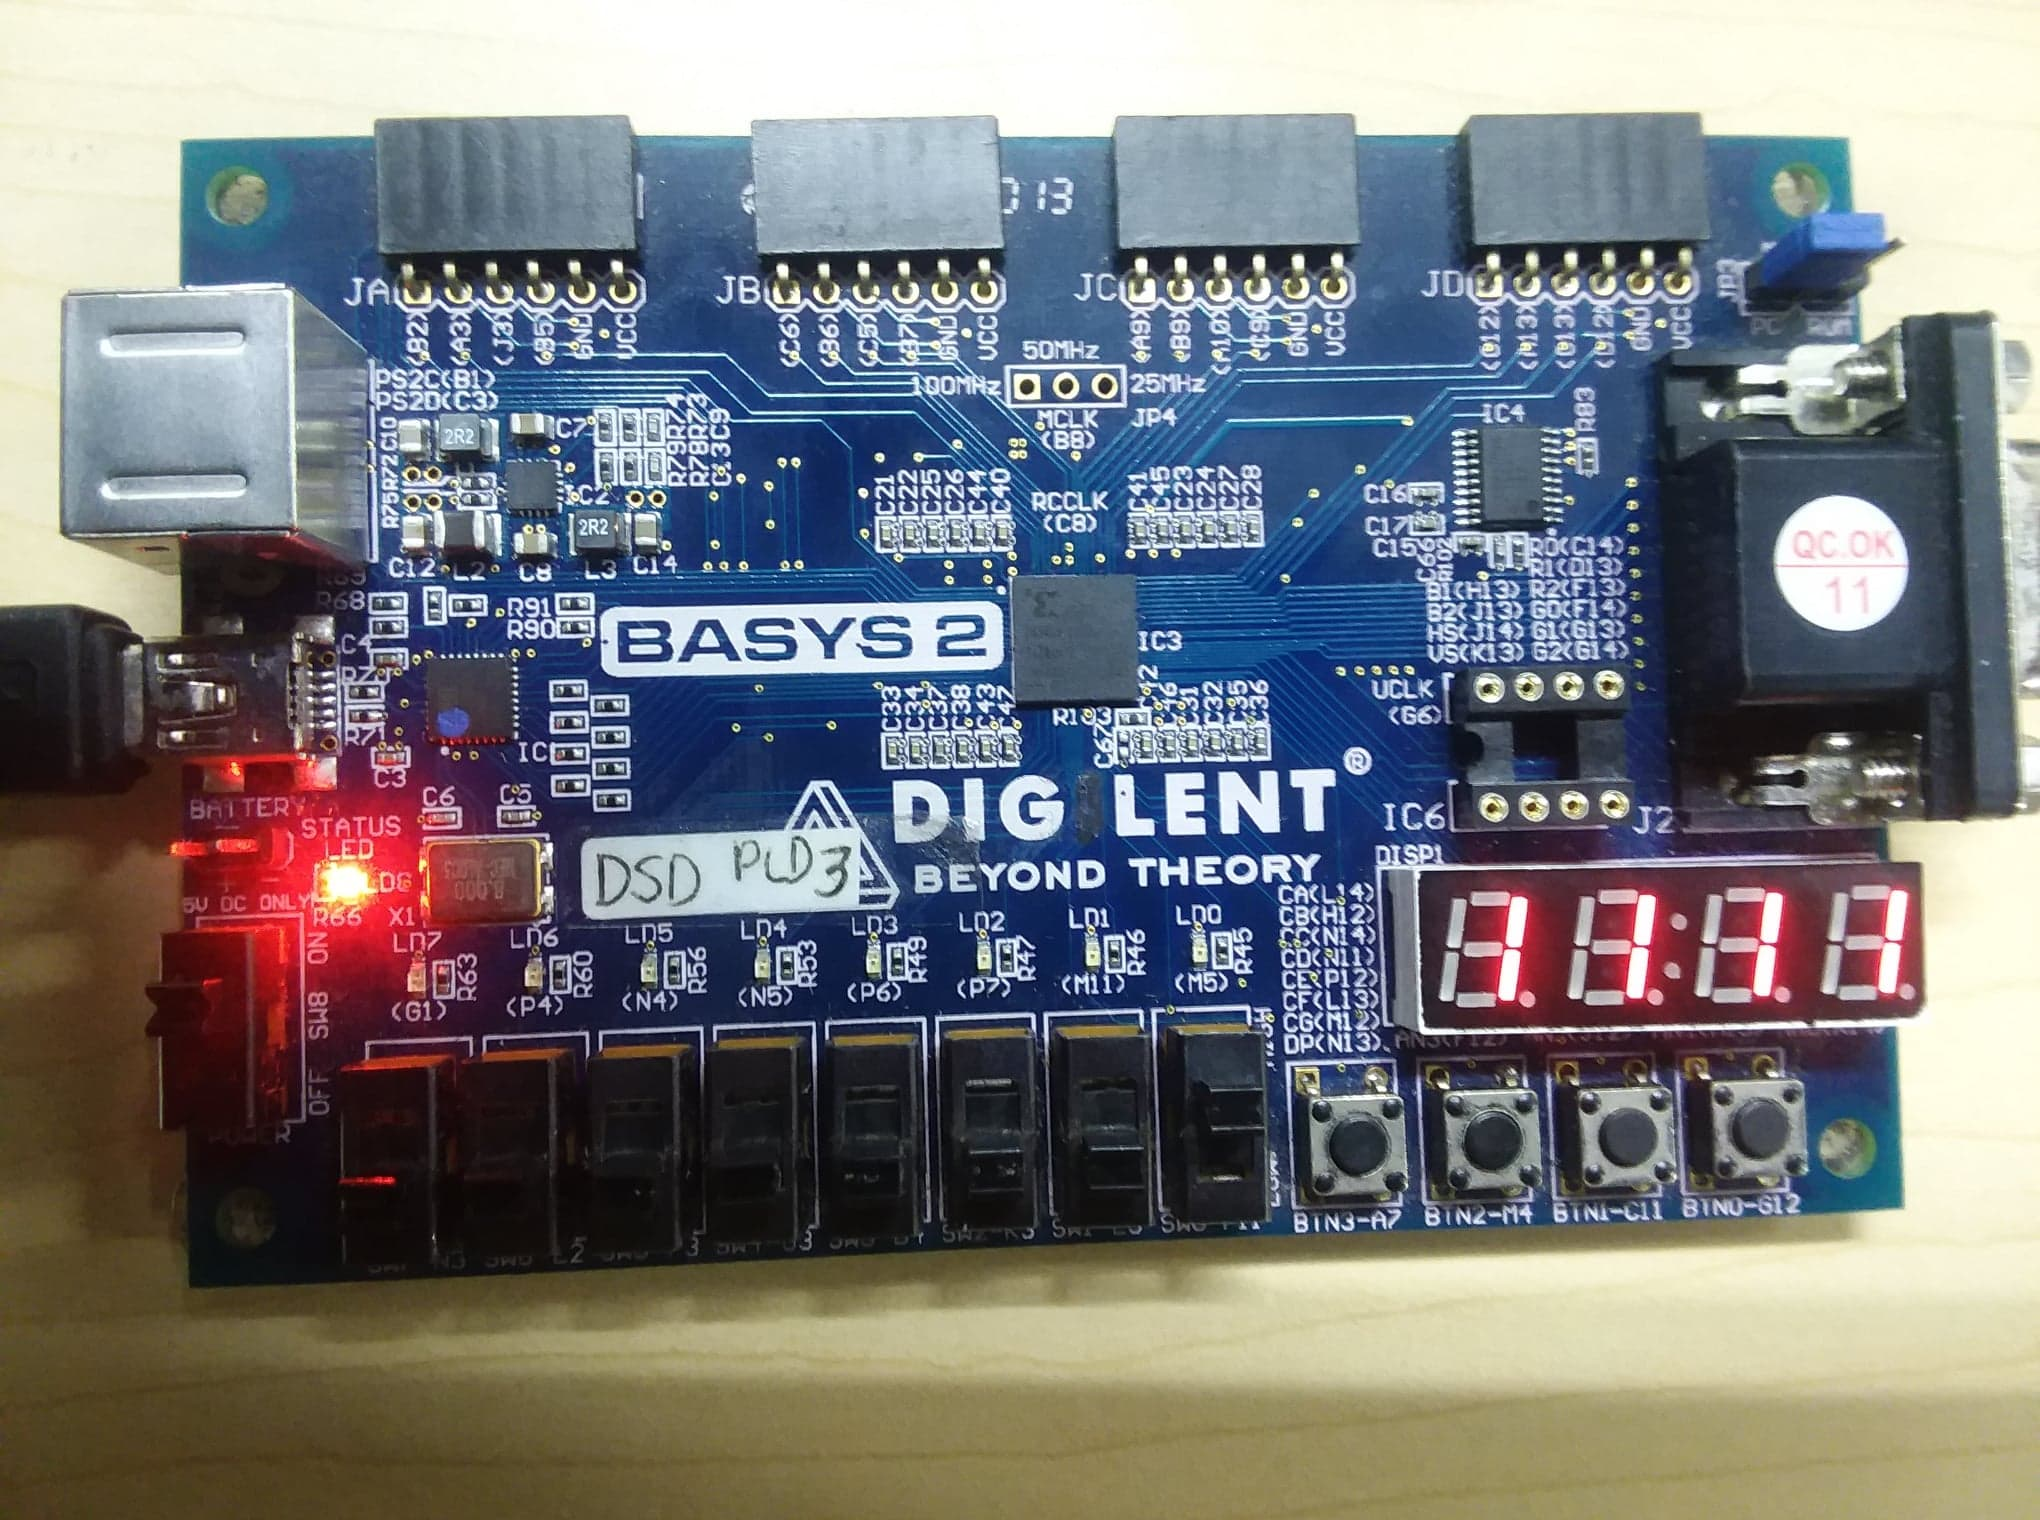
\includegraphics[width=7cm]{01} }}%
    \caption{Display de 7 segmento controlado por un decodificador}%
    \label{fig:example}%
\end{figure}

\begin{figure}[H]%
    \centering
    \subfloat[Dos]{{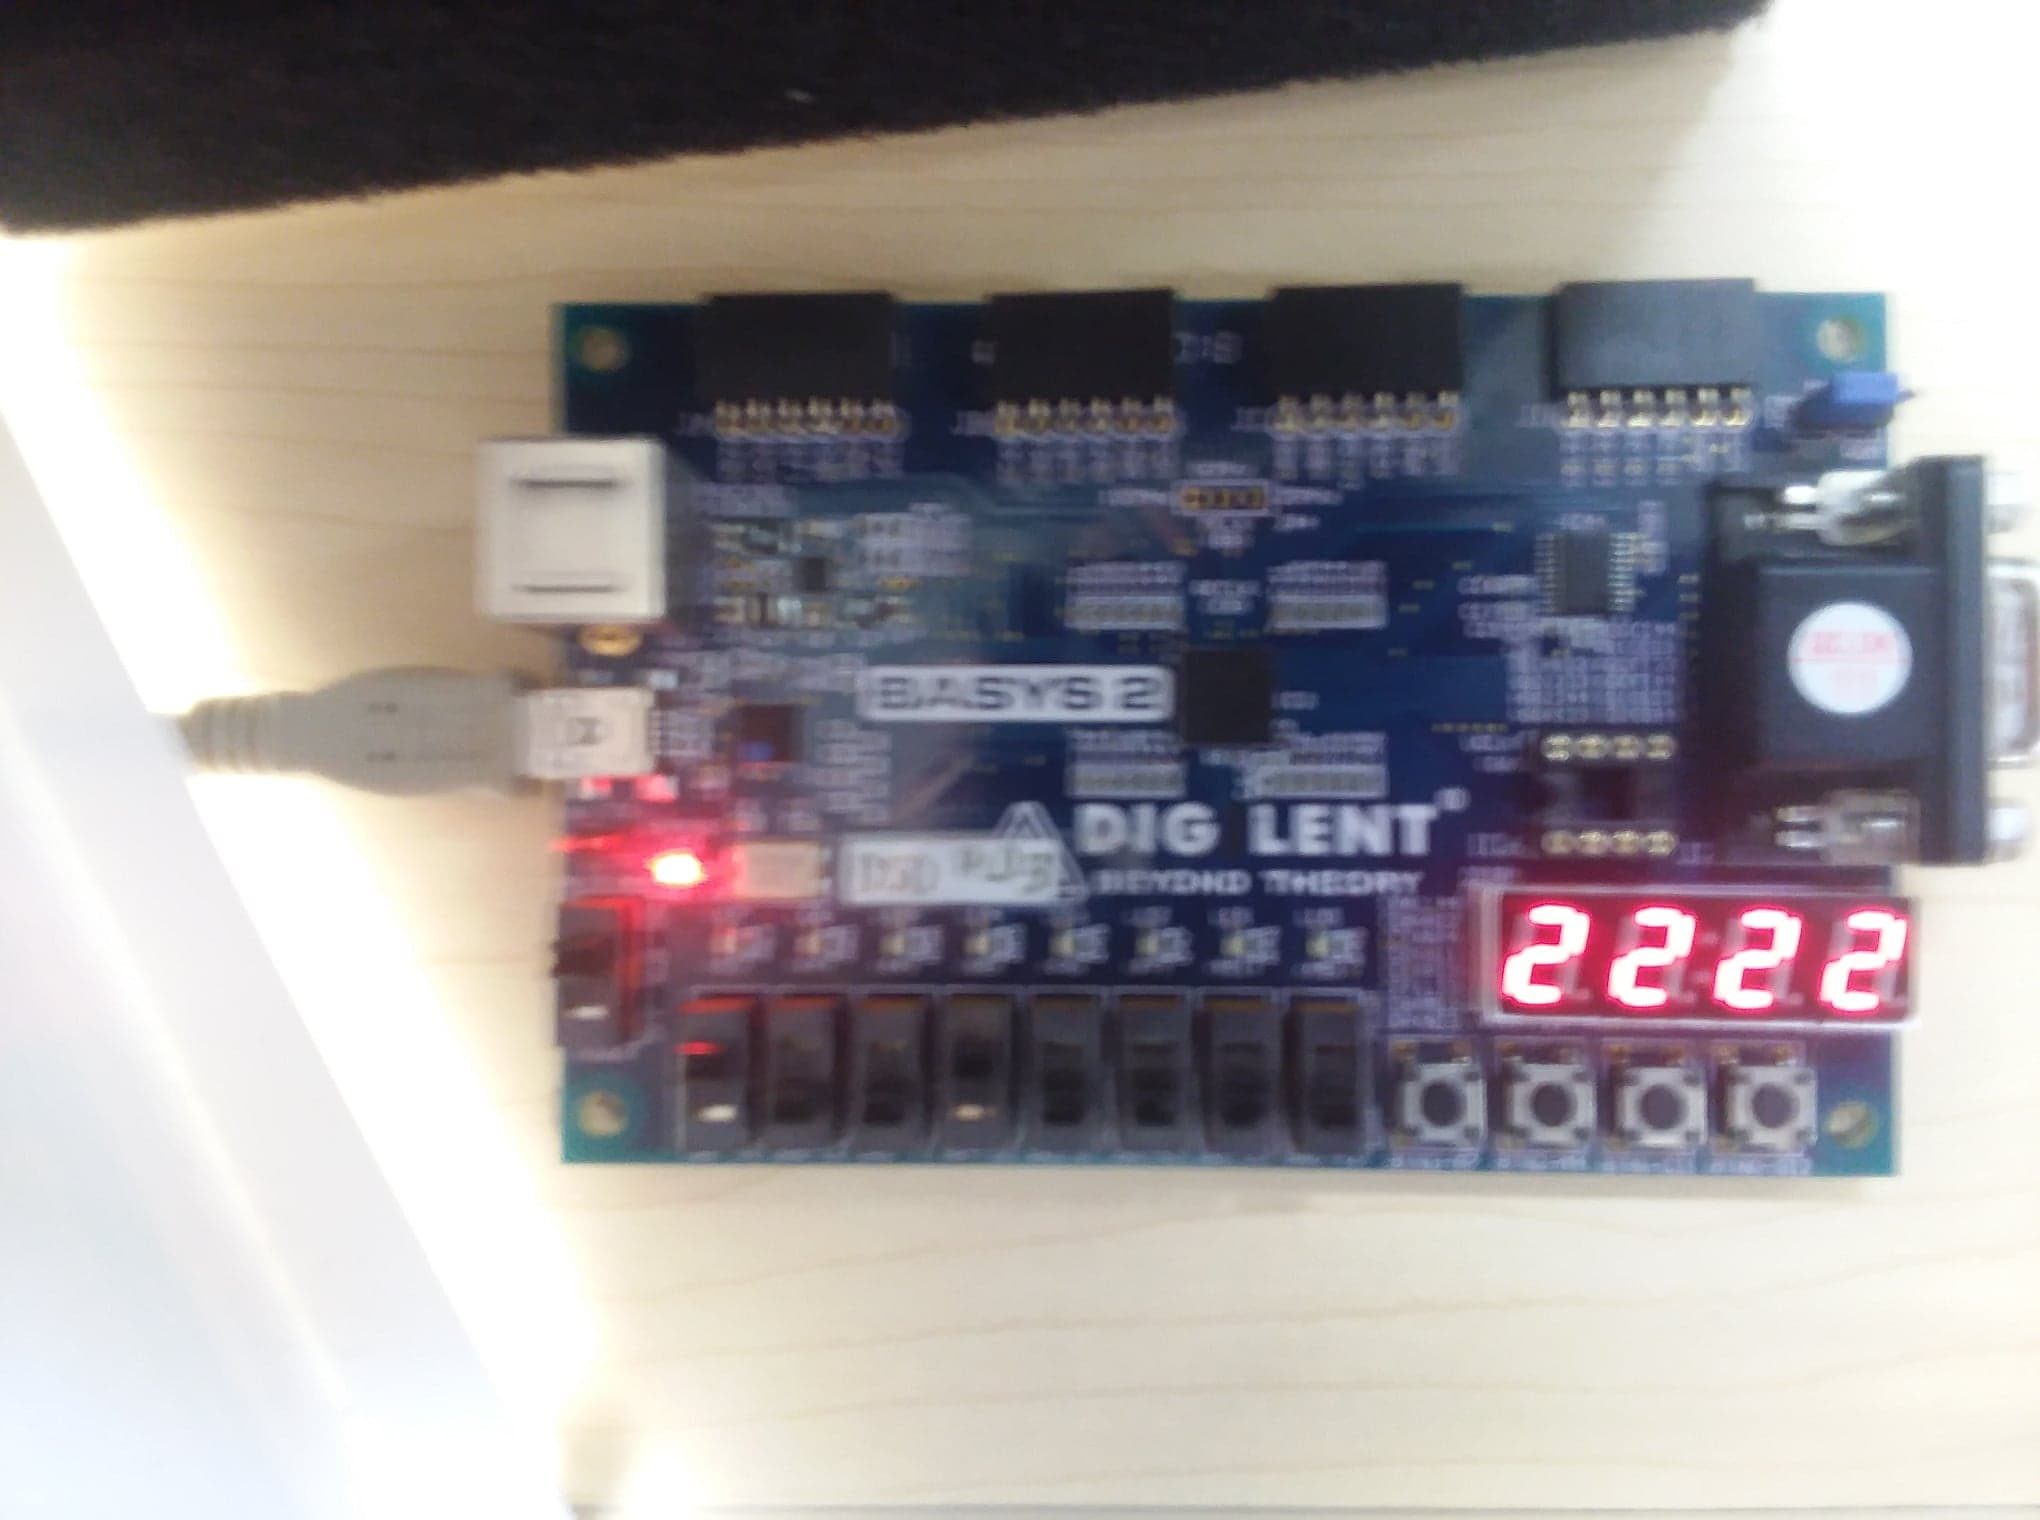
\includegraphics[width=7cm]{02} }}%
    \qquad
    \subfloat[Tres]{{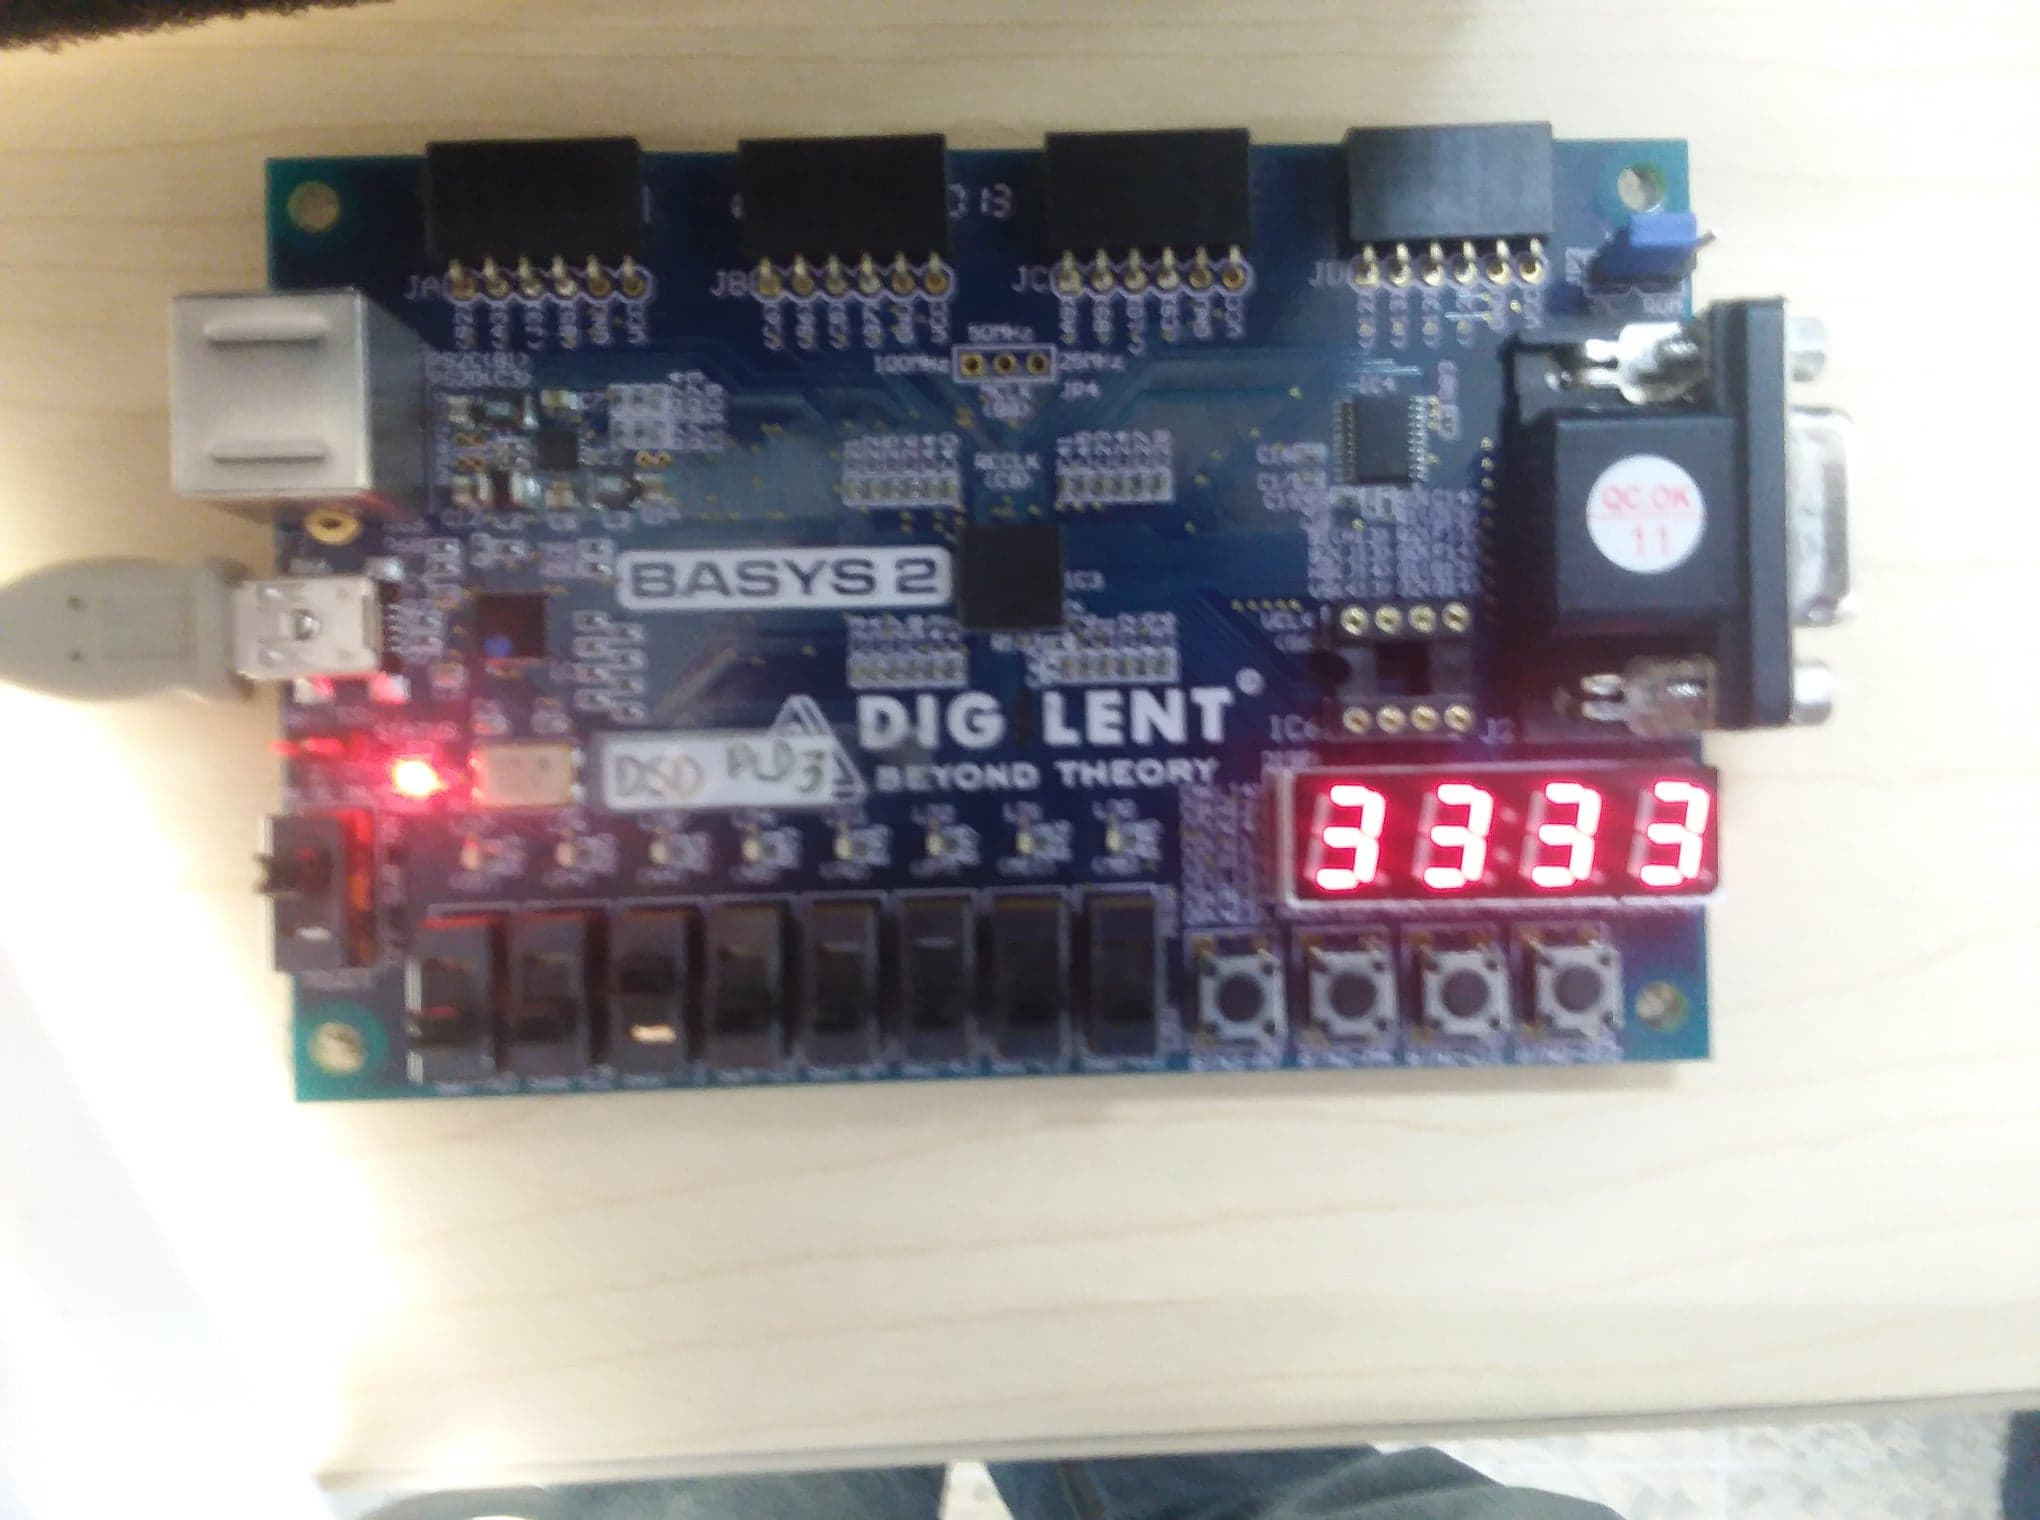
\includegraphics[width=7cm]{03} }}%
    \caption{Display de 7 segmento controlado por un decodificador}%
    \label{fig:example}%
\end{figure}

\begin{figure}[H]%
    \centering
    \subfloat[Cuatro]{{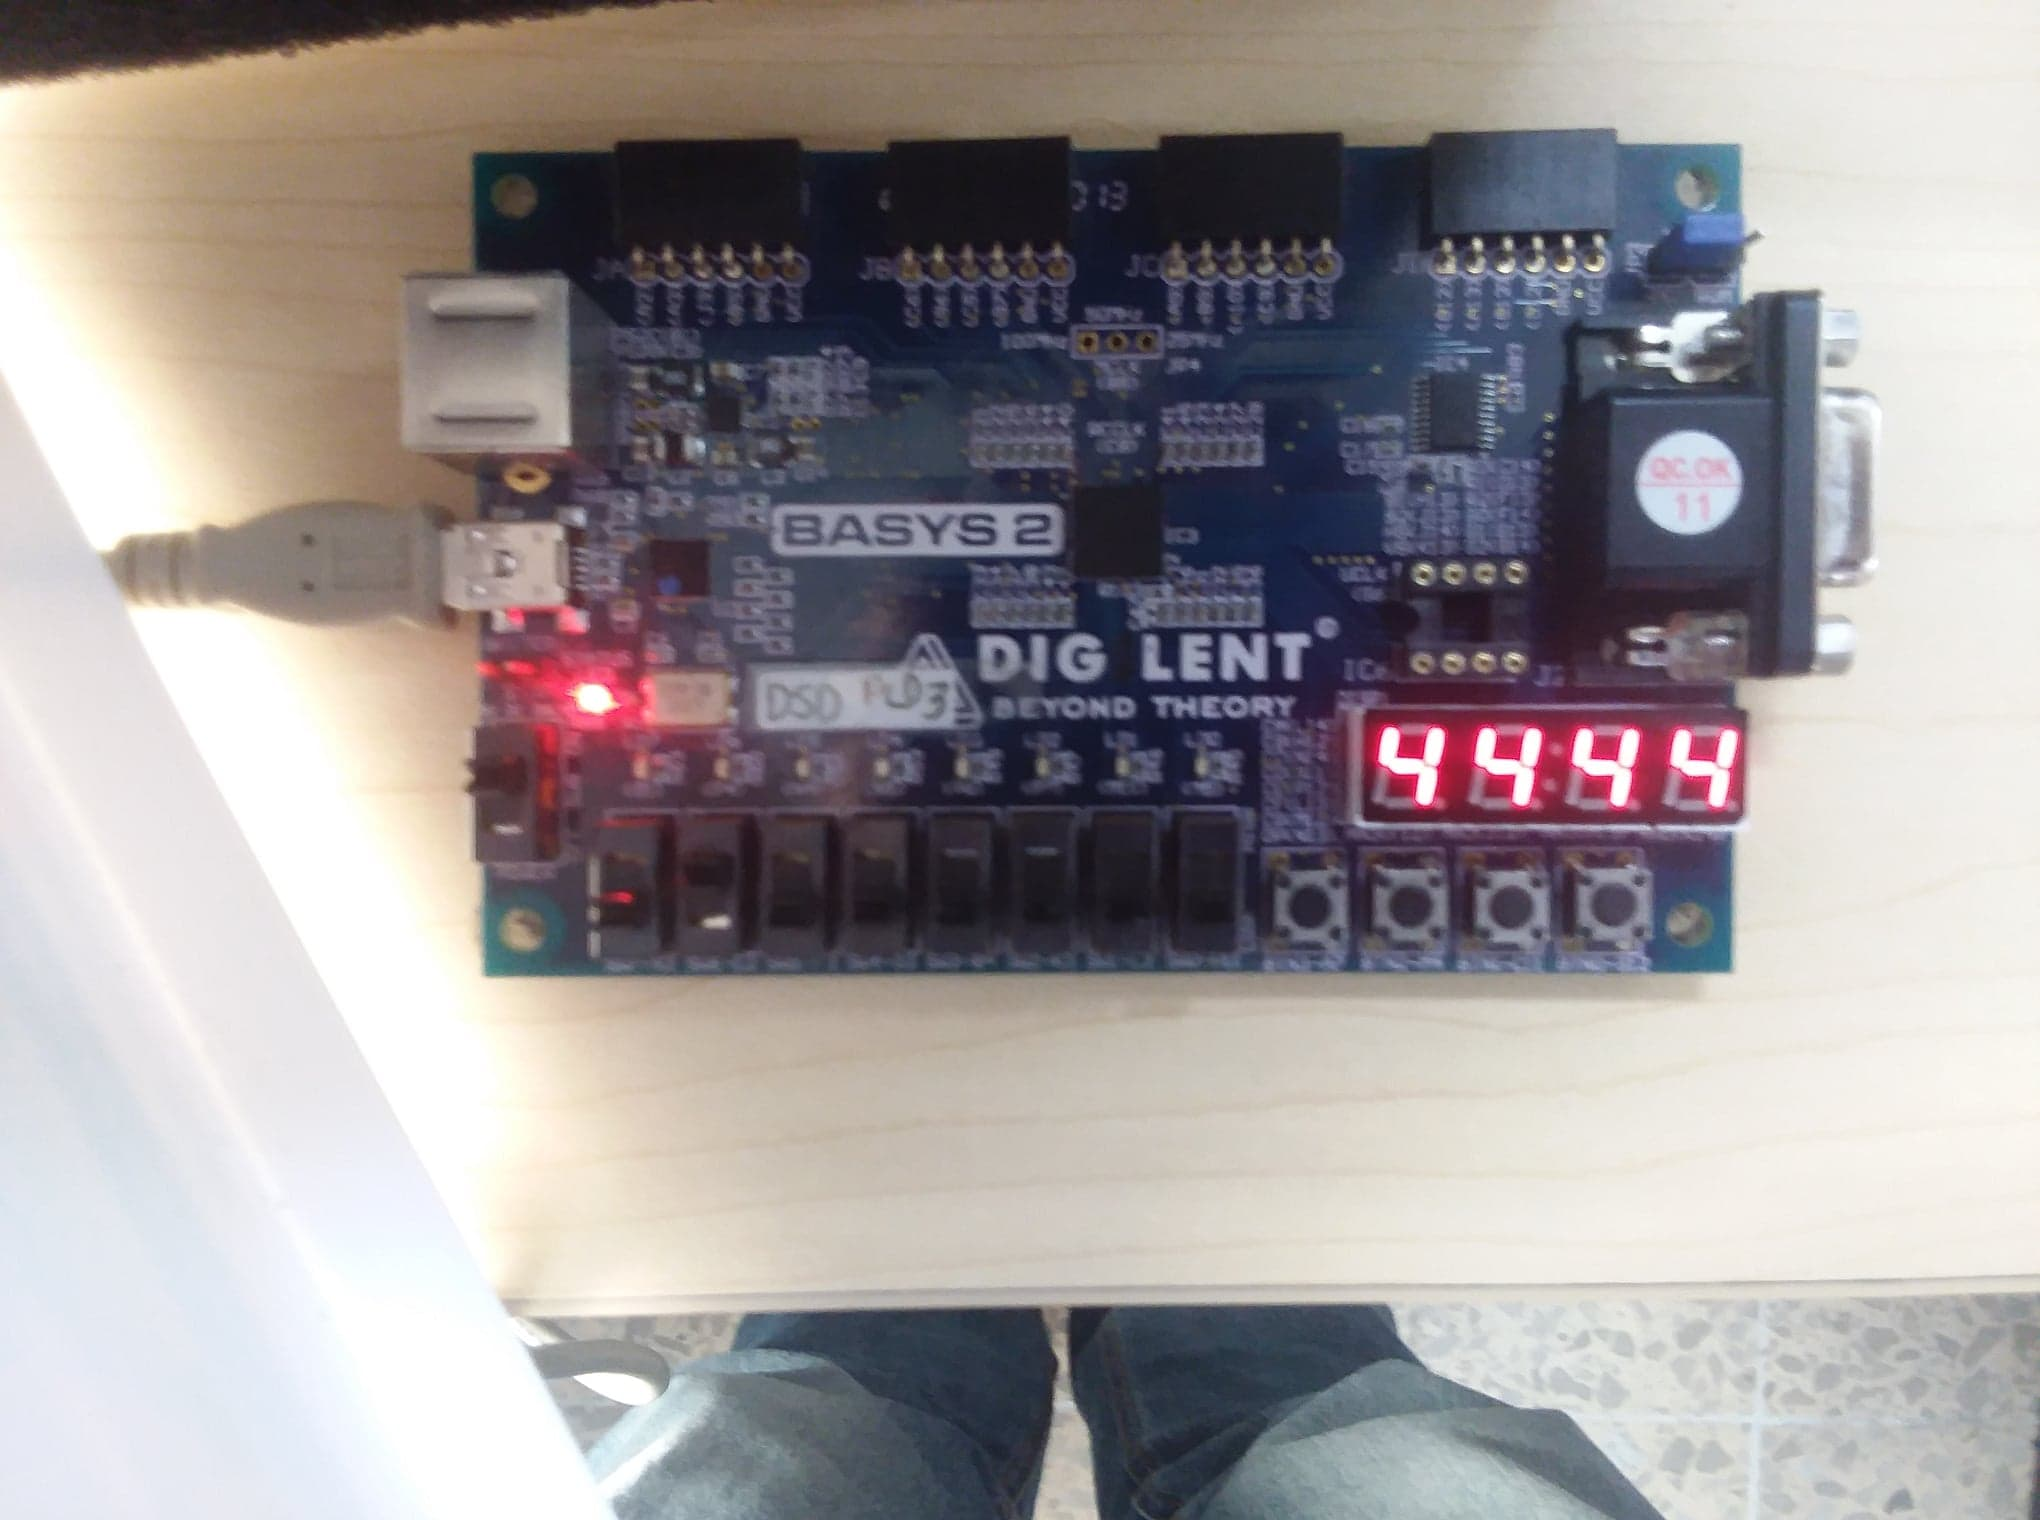
\includegraphics[width=7cm]{04} }}%
    \qquad
    \subfloat[Cinco]{{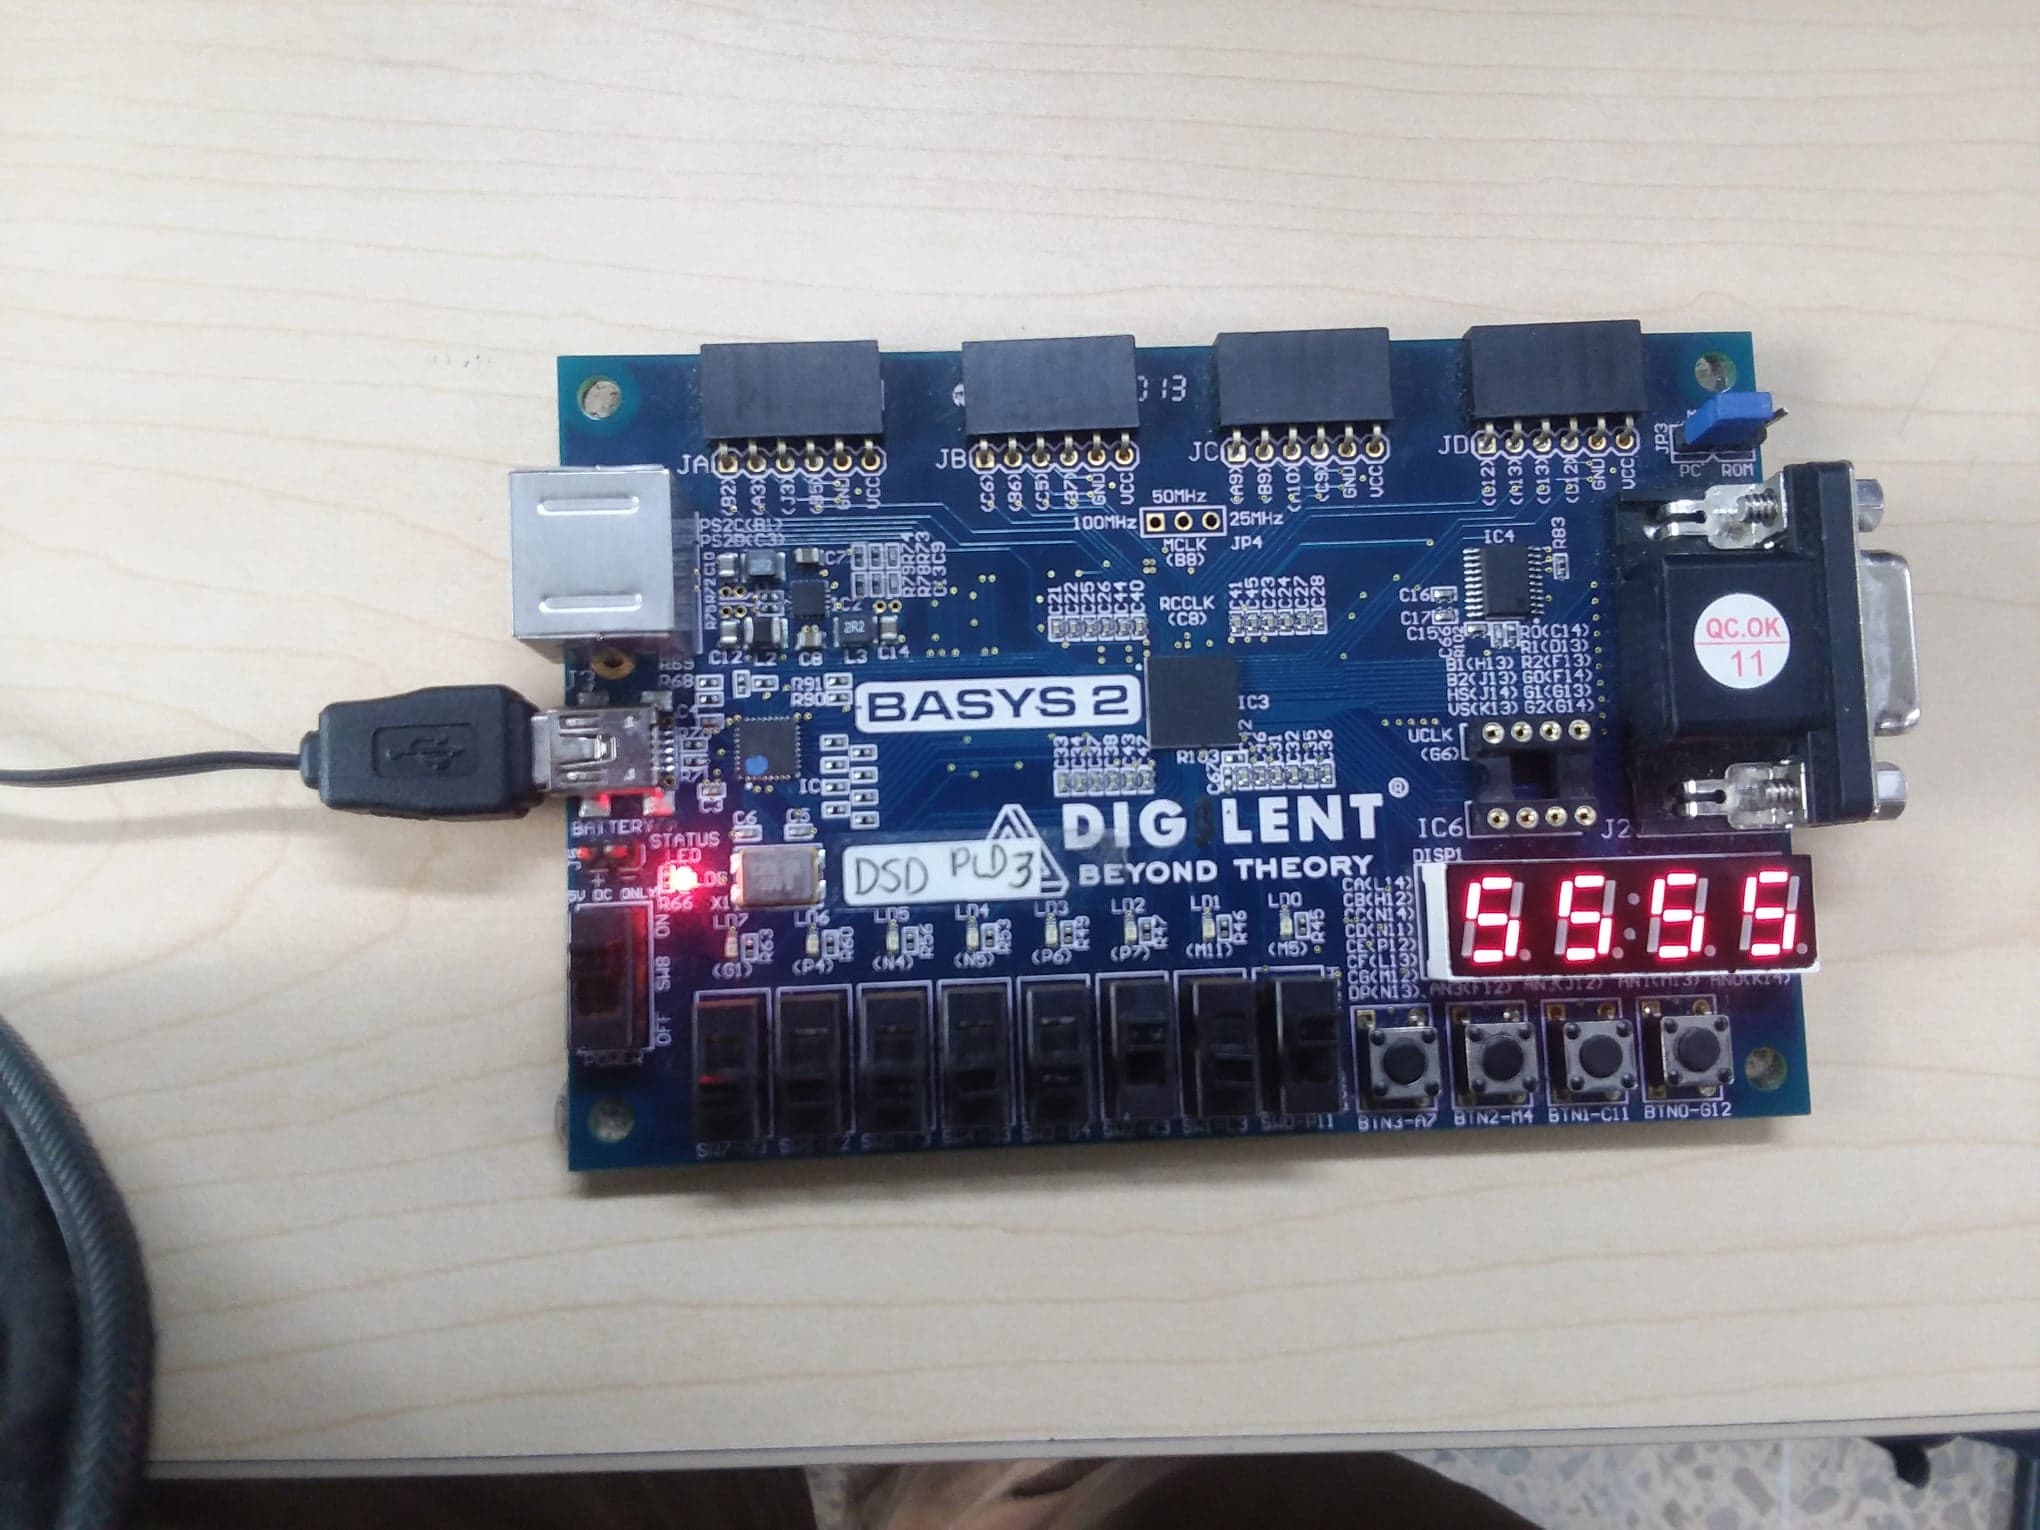
\includegraphics[width=7cm]{05} }}%
    \caption{Display de 7 segmento controlado por un decodificador}%
    \label{fig:example}%
\end{figure}

\begin{figure}[H]%
    \centering
    \subfloat[Seis]{{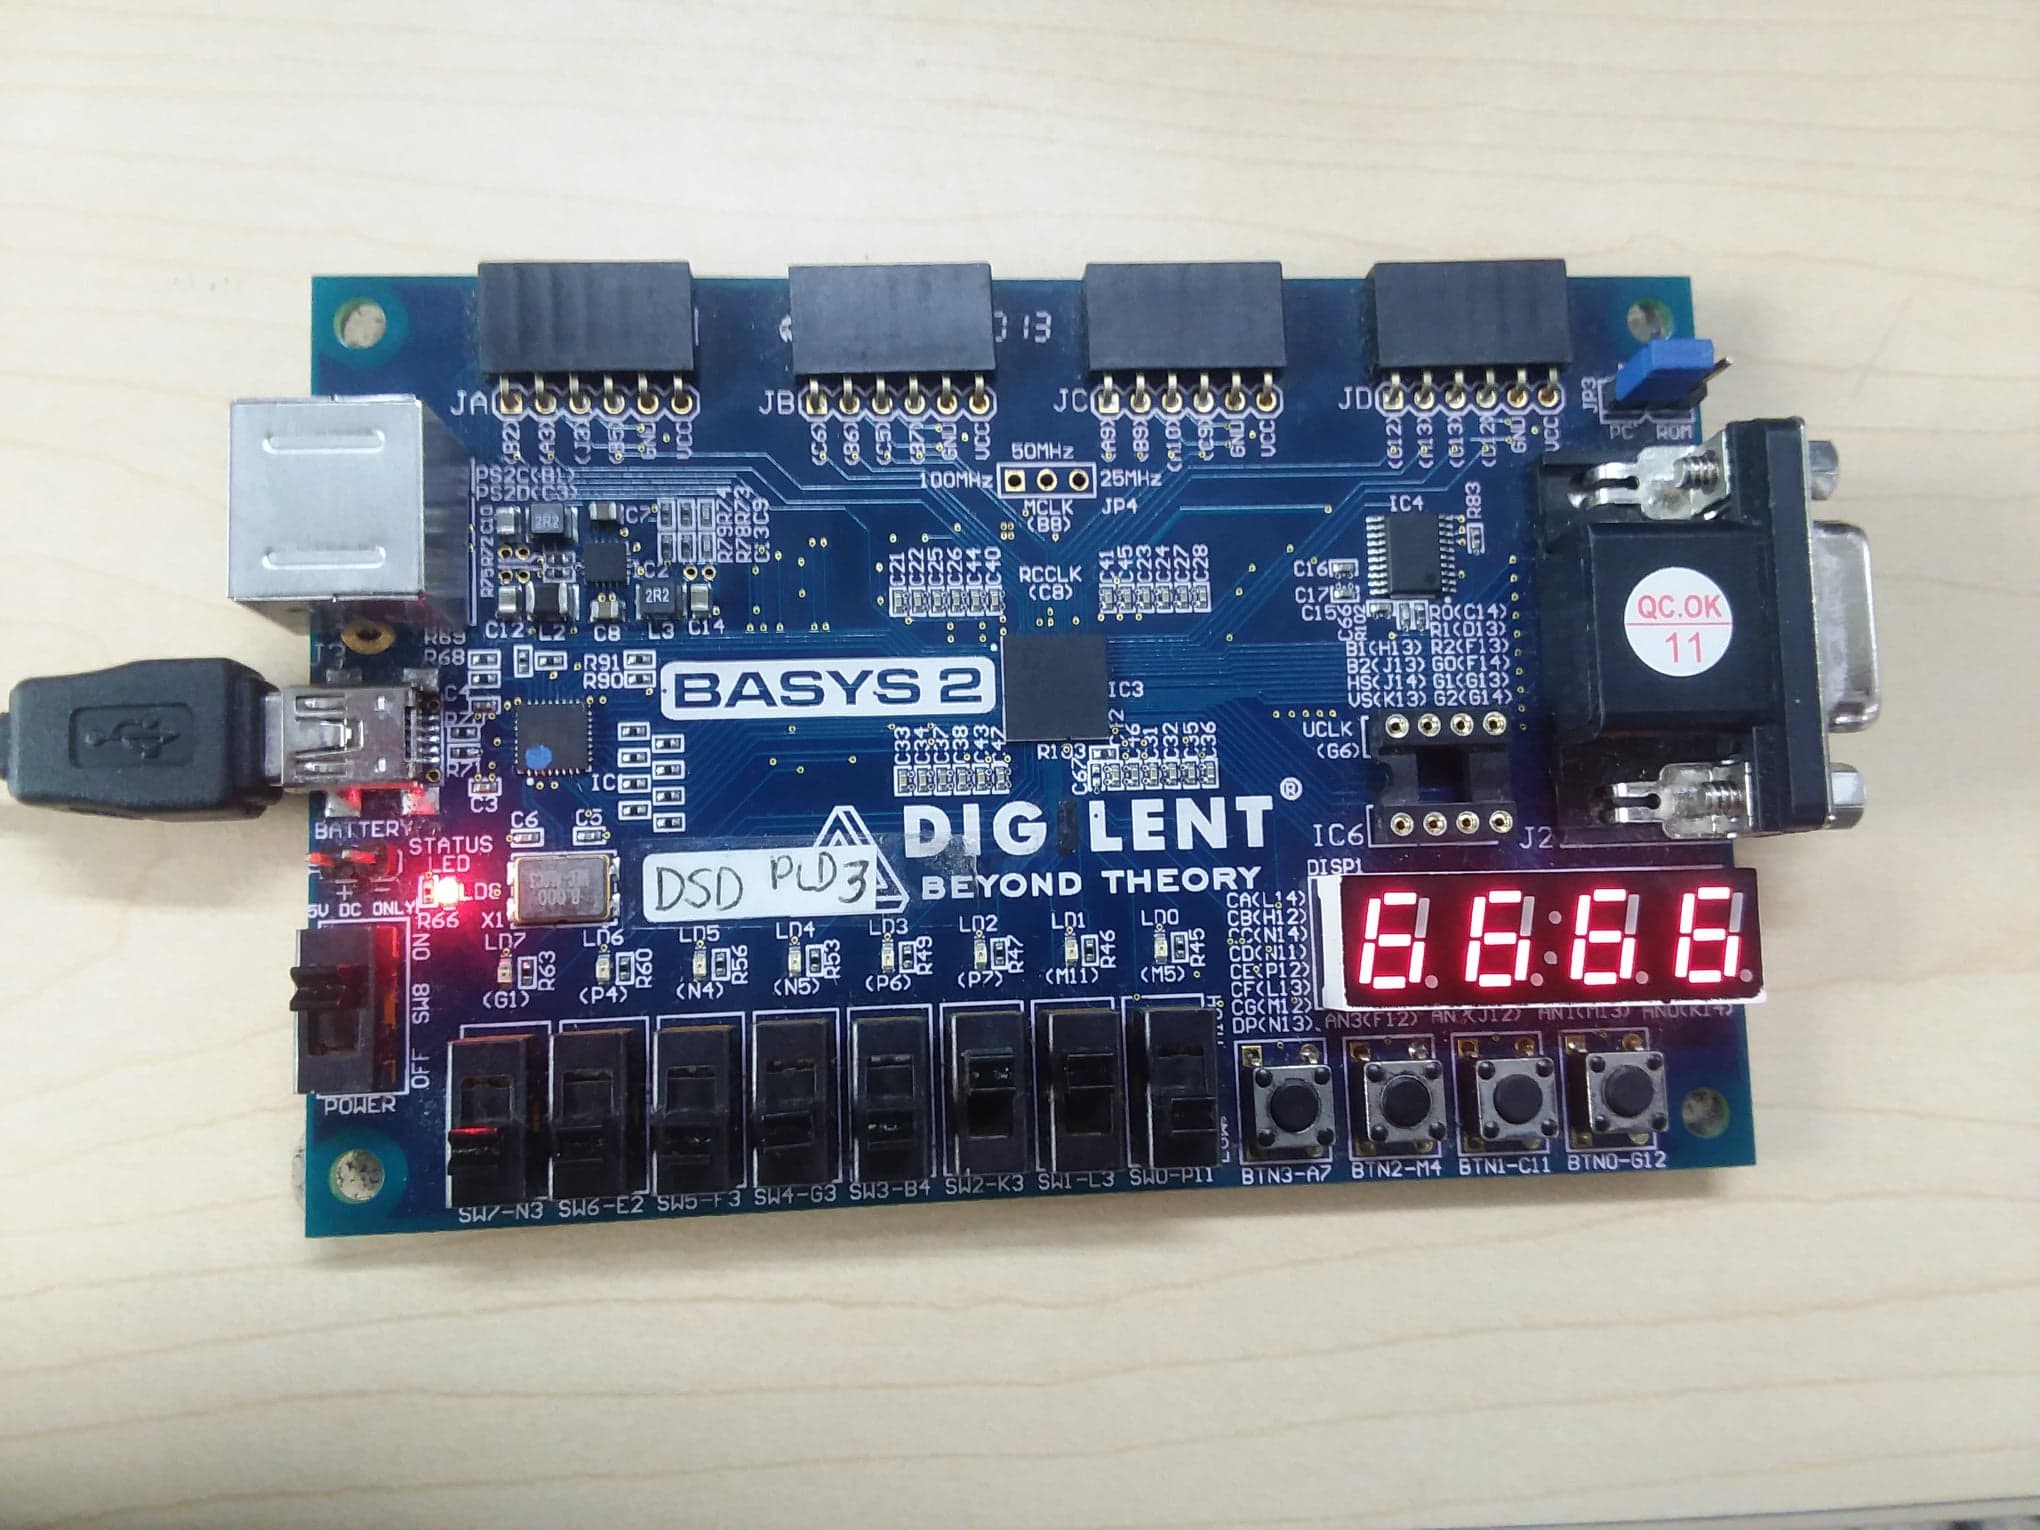
\includegraphics[width=7cm]{06} }}%
    \qquad
    \subfloat[Siete]{{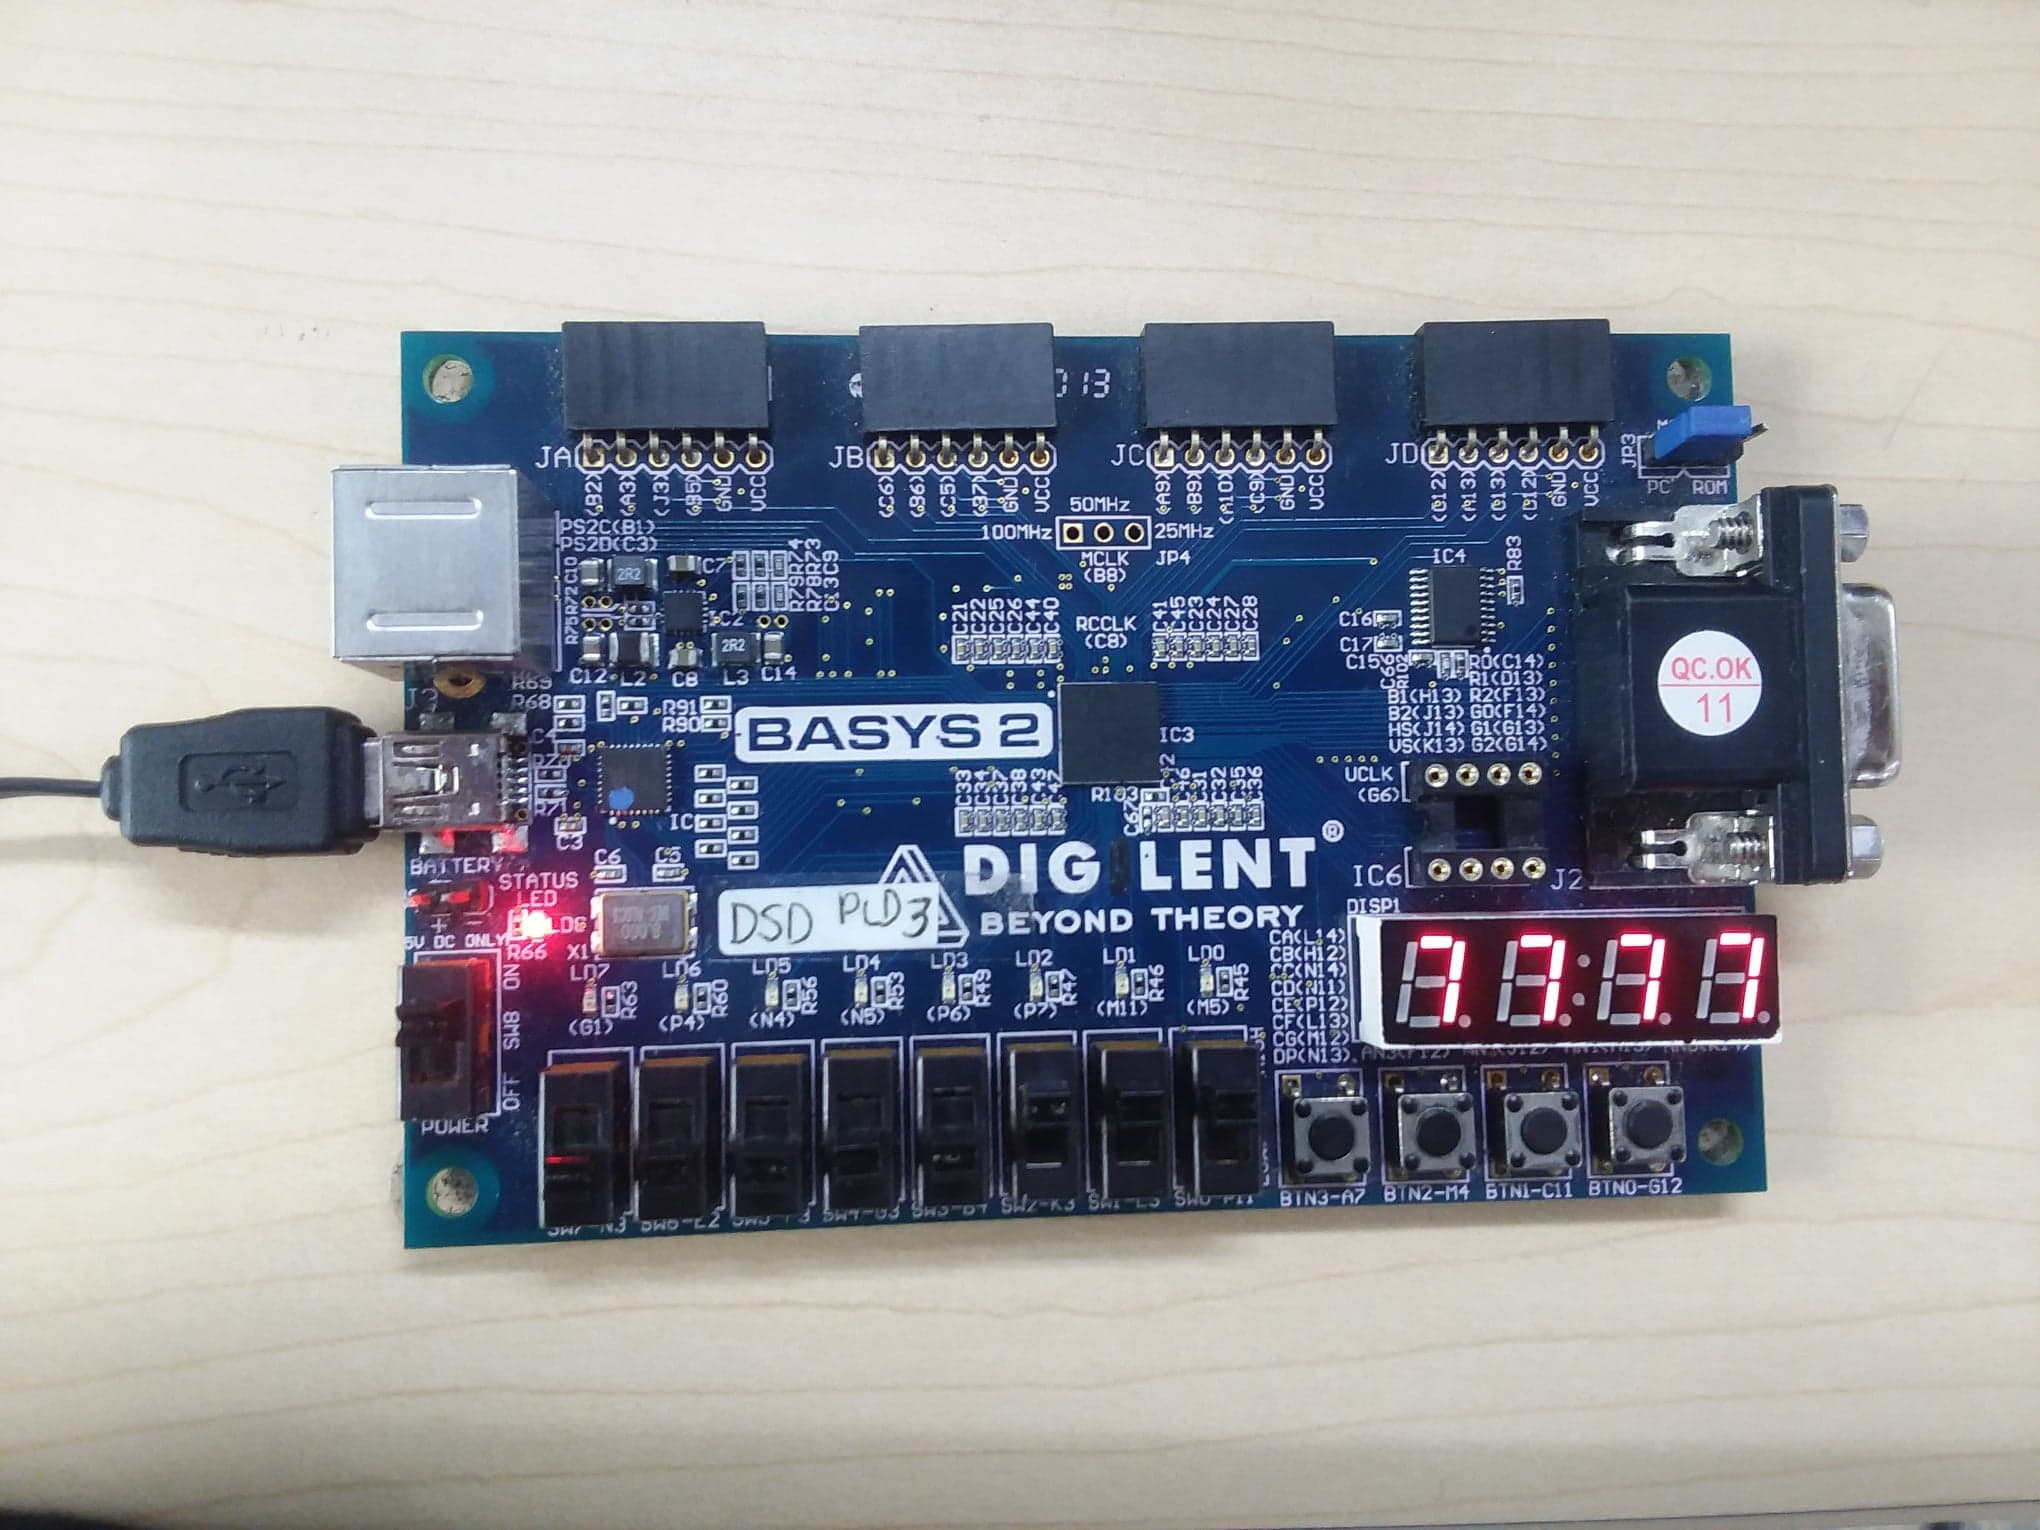
\includegraphics[width=7cm]{07} }}%
    \caption{Display de 7 segmento controlado por un decodificador}%
    \label{fig:example}%
\end{figure}

\begin{figure}[H]%
    \centering
    \subfloat[Ocho]{{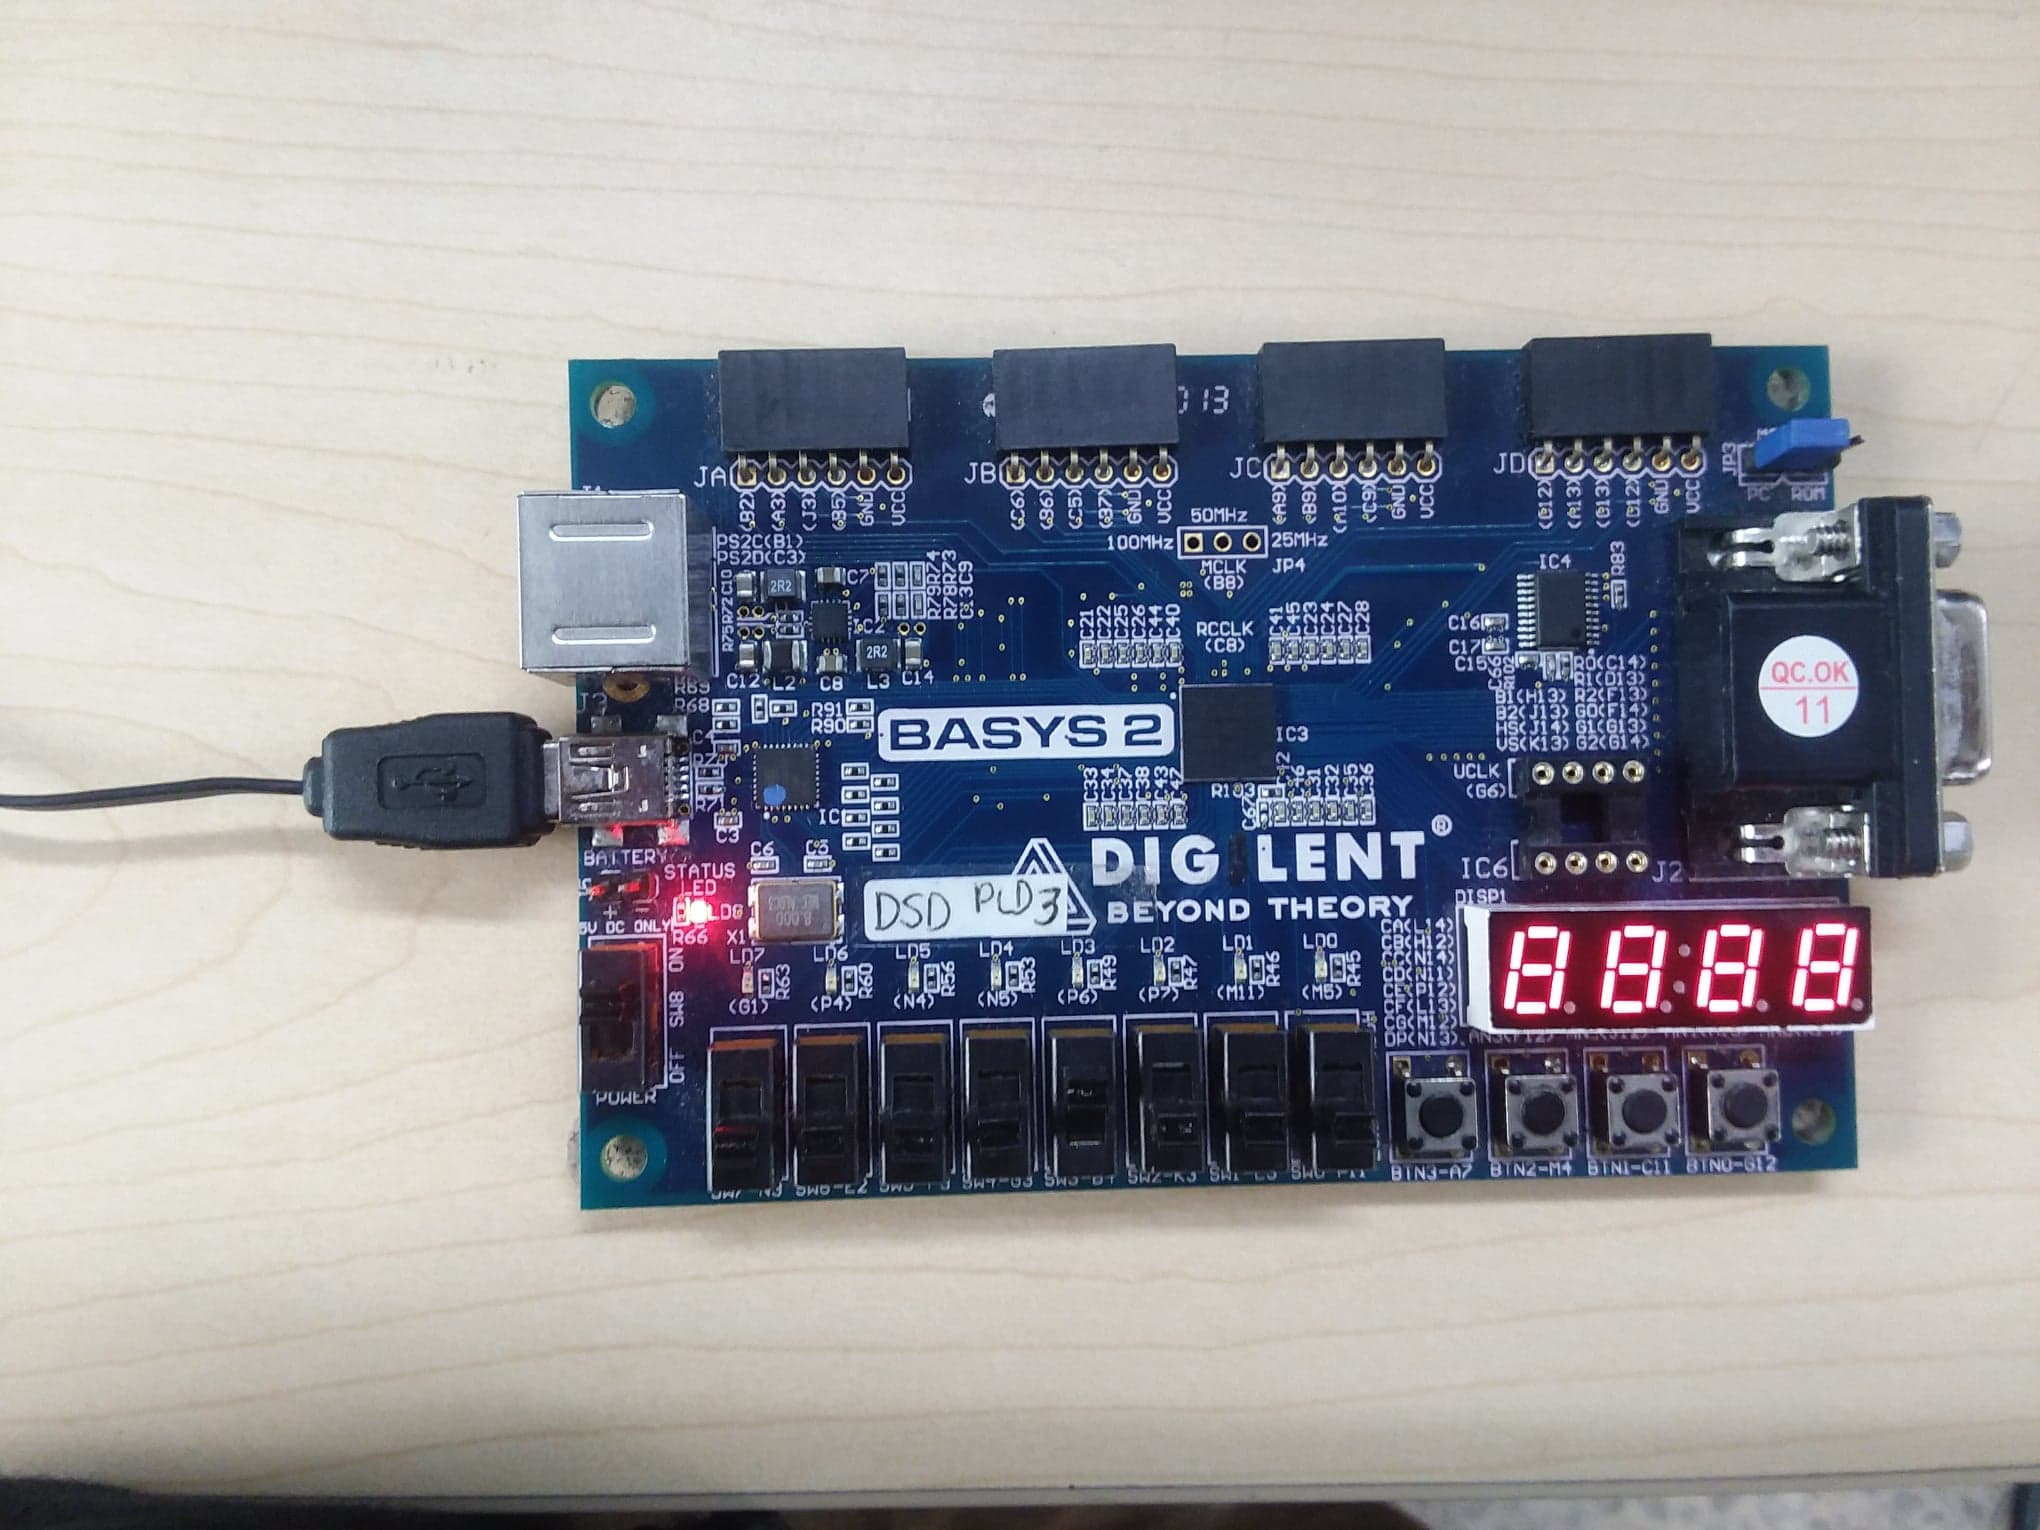
\includegraphics[width=7cm]{08} }}%
    \qquad
    \subfloat[Nueve]{{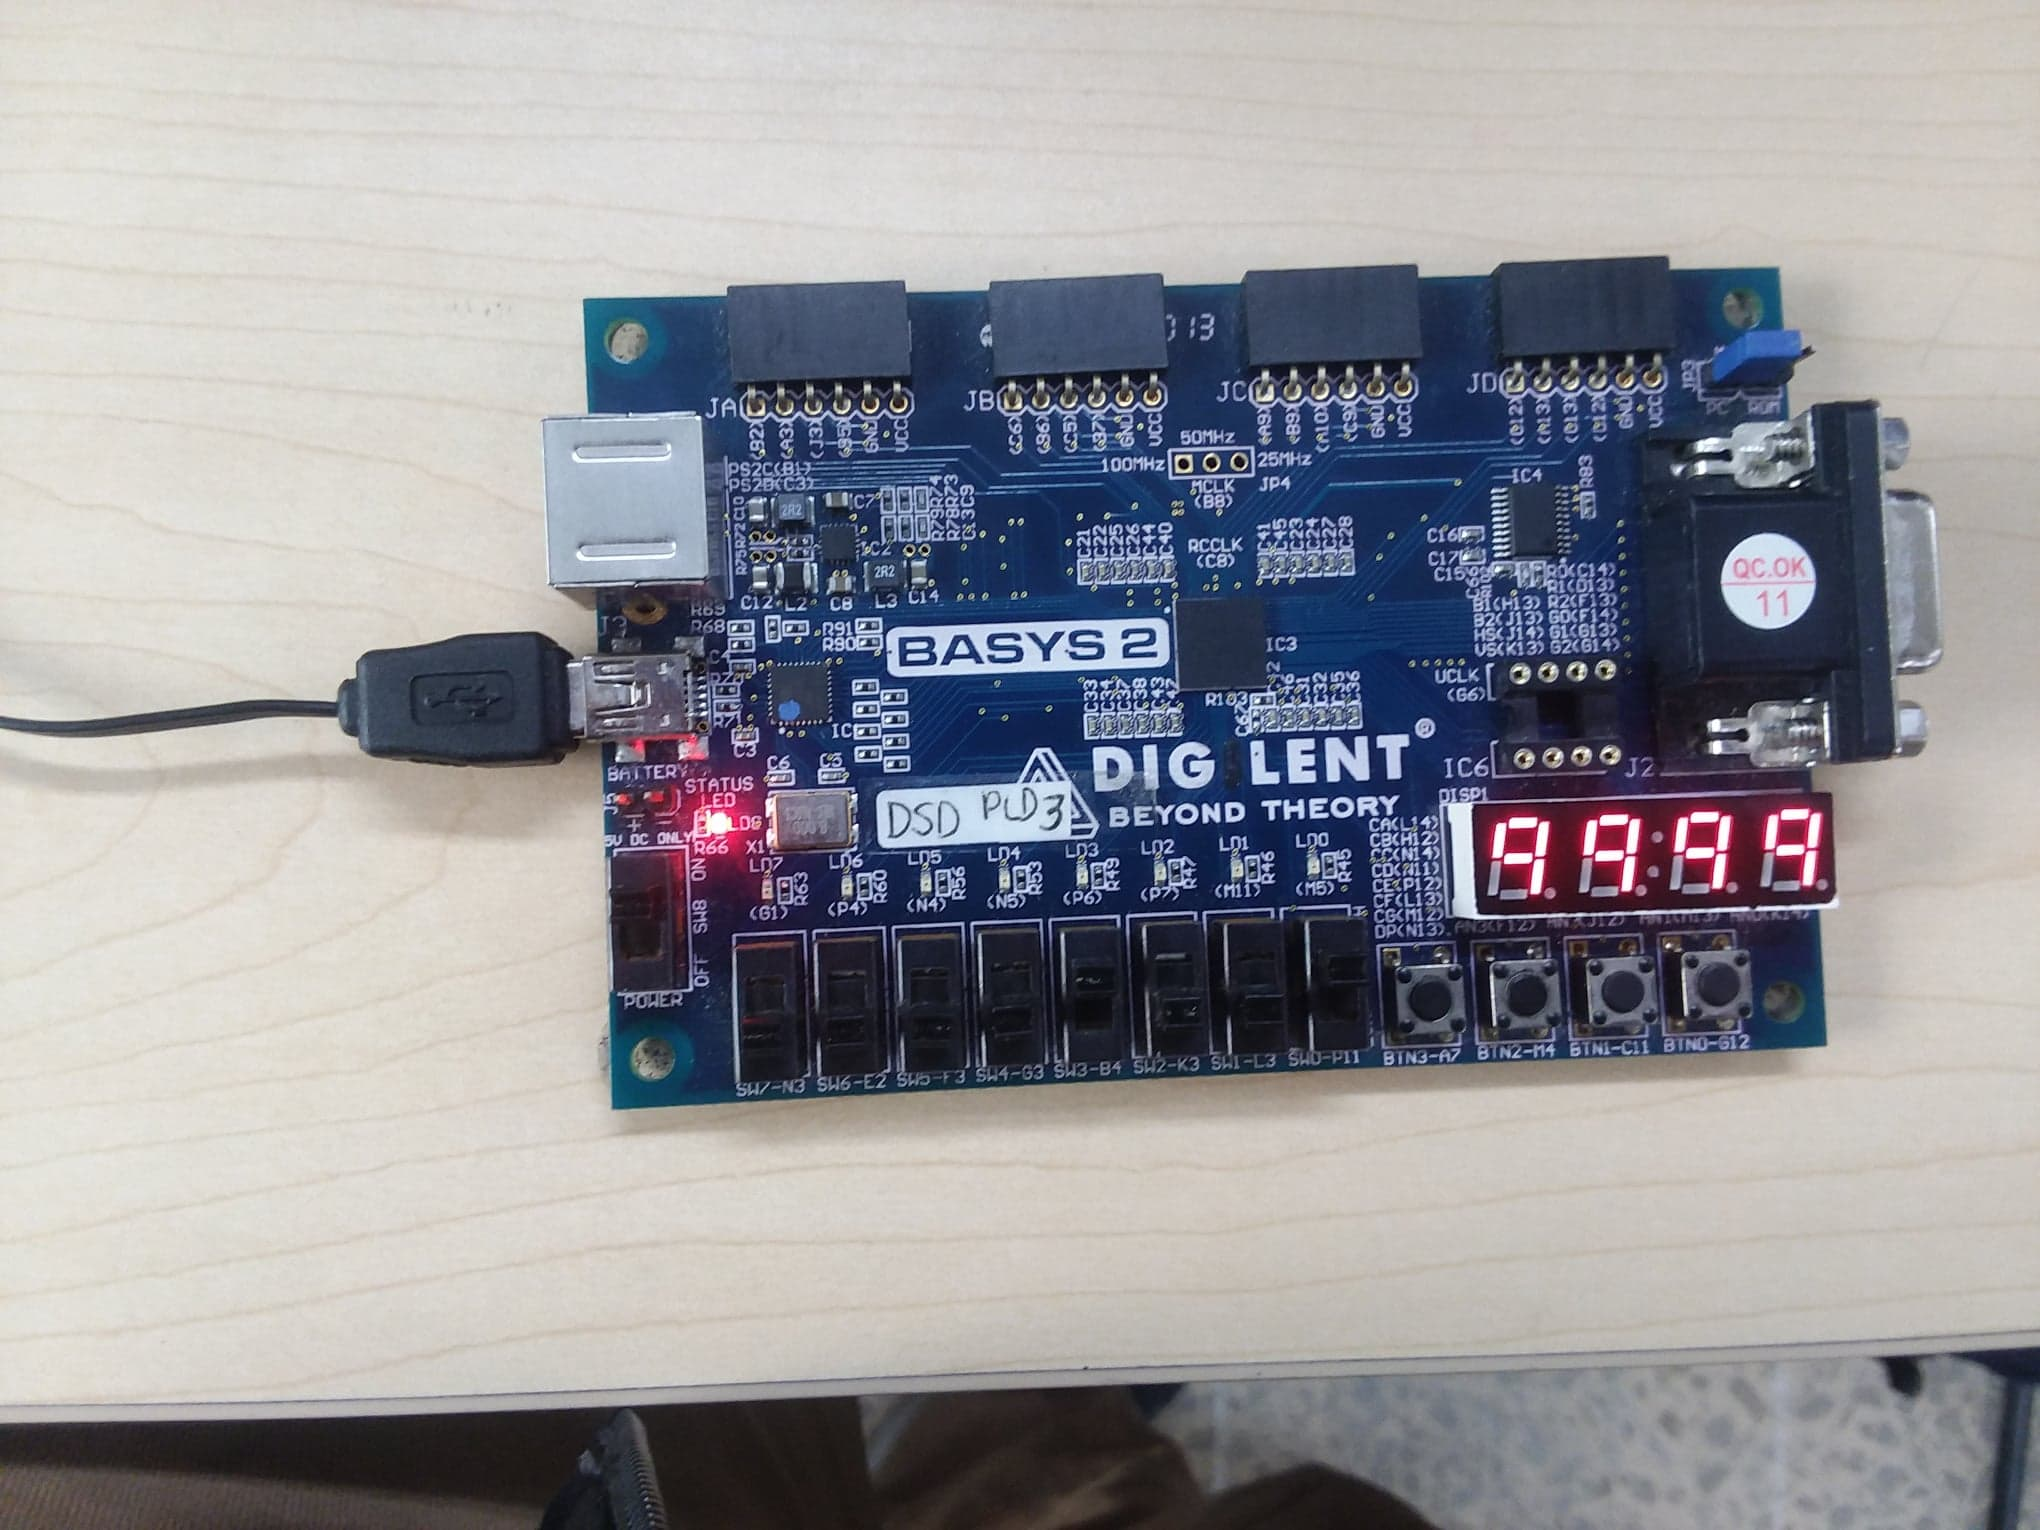
\includegraphics[width=7cm]{09} }}%
    \caption{Display de 7 segmento controlado por un decodificador}%
    \label{fig:example}%
\end{figure}

\section{Conclusiones}

Observamos que se puede se puede representar cualquier función booleana, para este caso, el código de 7 segmentos. Dicha función booleana puede ser representada con 1 decodificador de 4x16 pero para hacer más interesante la práctica demostramos que se puede controlar el display con \textbf{dos decodificadores} de 3x8 con señal \textit{enable}.

Para la implementación de este circuito en VHDL usamos el diseño esquemático pero antes tuvimos que crear en código VHDL los decodificadores de 3x8, para ello simplemente utilización la función de minitérminos.

\end{document}
